\documentclass[11pt,a4paper]{article}
\usepackage{amsmath,amssymb,booktabs,array,graphicx}
\usepackage[margin=2.35cm]{geometry}
\usepackage{microtype,float}
\usepackage[hidelinks]{hyperref}
\setlength{\emergencystretch}{2em}
\newcommand{\Euc}{\mathrm{Euc}}
\newcommand{\dec}{\mathrm{dec}}
\newcommand{\nr}{\mathrm{nr}}
\newcommand{\Flim}{F_{\mathrm{lim}}}
\newcommand{\Lref}{L_{\mathrm{ref}}}
\newcommand{\Ldec}{L_{\mathrm{dec}}}
\newcommand{\Lj}{L_{\mathrm j}}
\newcommand{\Lnr}{L_{\mathrm{nr}}}
\newcommand{\tcad}{t_{\mathrm{cad}}}
\newcommand{\tdec}{t_{\mathrm{dec}}}
\newcommand{\tj}{t_{\mathrm j}}
\newcommand{\tnr}{t_{\mathrm{nr}}}
\newcommand{\Rdet}{R_{\mathrm{det}}}
\newcommand{\ft}{\widetilde F_\nu}
\newcommand{\fp}{\widetilde F_p}
\graphicspath{{../analysis/simplified_luminosity_function/results/figures/}}
\title{\textbf{Simplified Luminosity Function}\\[5pt]
\large An explicit derivation and exploration of the detected population}
\author{}
\date{October 2026}
\begin{document}
\maketitle

\begin{abstract}
We replace the bounded luminosity distribution by a power-law event-rate
density extending over all positive luminosities. The purpose is to understand
which luminosities contribute to a survey and how the detection rate changes
with limiting flux, cadence, and the slope of the luminosity function.
We begin with the detectable volume of an event of luminosity $L$, derive
the luminosity and distance integrals in both orders, and then evaluate the
viewing-angle integral explicitly. This separates an exact result from the
project's most-contributing-point approximation. The same reasoning gives the
detected luminosity, distance, and angle distributions, and explains precisely
when the threshold at $D_\Euc$ is a useful characteristic luminosity.
The final steps connect the result to repeated detections and to the original
bounded luminosity function. Only a few numerical examples are retained to
illustrate the analytic behavior.
\end{abstract}

\section{What is being simplified?}
\label{sec:population}
The previous derivation~\cite{PreviousLF} distributes the on-axis spectral luminosity at the
deceleration time,
\begin{equation}
 L\equiv L_\nu(\tdec),\qquad [L]=\mathrm{erg\,s^{-1}\,Hz^{-1}}.
 \label{eq:Ldefinition}
\end{equation}
It specifies a total intrinsic rate and a normalized luminosity distribution
between $L_{\min}$ and $L_{\max}$. Here we specify directly how many events
occur in each luminosity interval, per unit volume and time:
\begin{equation}
 \boxed{\frac{d\mathcal R}{dL}
 =\frac{\mathcal A}{\Lref}\left(\frac L{\Lref}\right)^\alpha,
 \qquad 0<L<\infty,\qquad
 \Lref=10^{32}\,\mathrm{erg\,s^{-1}\,Hz^{-1}}.}
 \label{eq:intensity}
\end{equation}
The two adjustable population parameters are $\mathcal A$ and $\alpha$.
The reference luminosity $\Lref$ is fixed; it is a convention for quoting
$\mathcal A$, not another physical luminosity scale. Multiplying by $L$ gives
\begin{equation}
 \frac{d\mathcal R}{d\ln L}
 =\mathcal A\left(\frac L{\Lref}\right)^{\alpha+1},
 \qquad
 \left.\frac{d\mathcal R}{d\ln L}\right|_{L=\Lref}=\mathcal A.
 \label{eq:logintensity}
\end{equation}
Thus $\mathcal A$ is the volumetric event rate per natural-log luminosity
interval at $\Lref$. It can be quoted in $\mathrm{Gpc^{-3}\,yr^{-1}}$.
The power-law index is defined \emph{per unit luminosity}: per logarithmic
interval the index is $\alpha+1$. We keep this distinction throughout.

We use the notation of the thesis and the previous LF derivation. In
particular $D_\Euc$ is the Euclidean radius, $q=\theta_{\rm obs}/\theta_j$
is the viewing angle in units of the jet half-angle, $\Flim$ is the spectral
limiting flux, and $i$ is the required number of detections. The physical
luminosity thresholds $\Ldec,\Lj,\Lnr,L_i$, and $L_\Euc(q)$ are defined as
we encounter them. No auxiliary angular integral or abbreviated exponent is
needed. All rates below are all-sky rates; a uniform surveyed solid angle
multiplies them by its fraction of $4\pi$.

The equations use consistent length units. For example, if luminosities and
fluxes are in cgs units, use distances in cm and convert the quoted
$\mathcal A$ from $\mathrm{Gpc^{-3}\,yr^{-1}}$ to
$\mathrm{cm^{-3}\,yr^{-1}}$ before multiplying by a volume in $\mathrm{cm^3}$.
This conversion is understood whenever $4\pi D^2\Flim$ and $D^3\mathcal A$
appear together.

\subsection{What remains the same as in the project}
The source population is uniform in Euclidean volume, with random jet
orientations and a common afterglow light-curve shape. Changing $L$ multiplies
the entire light curve without changing $p$, $\Gamma_0$, $\theta_j$,
$\tdec$, or $\tj$. Here $p$ is the electron-energy power-law index of the
project; it is not a probability-density symbol. The model is therefore a
brightness distribution at fixed dynamics. Correlations between luminosity
and duration, jet opening angle, or spectral evolution would require a further
extension.

\subsection{Why there is no finite total intrinsic rate}
At low luminosity, $\int_0 L^\alpha dL$ is finite only for $\alpha>-1$.
At high luminosity, $\int^\infty L^\alpha dL$ is finite only for
$\alpha<-1$. No slope satisfies both conditions. Consequently
Eq.~\eqref{eq:intensity} is an event-rate density, not a normalized probability
distribution with a finite $R_{\rm int}$. Its total luminosity output is also
divergent: $\int_0^\infty L^{\alpha+1}dL$ has incompatible conditions at its
two ends.

The question is instead whether the \emph{detected} rate is finite. Very faint
sources occupy a very small detectable volume. That extra volume factor is
what can make the observation integral converge, despite the divergent
intrinsic population. We now derive it rather than assume it.

\section{From the light curve to a physical luminosity threshold}
\label{sec:threshold}
The thesis~\cite{Thesis} approximates an off-axis light curve as joining the on-axis
light curve at the peak time $t_p(q)$. The relevant angles and times are
\begin{gather}
 q_\dec=1+\frac1{\Gamma_0\theta_j},\qquad
 q_{\rm j}=2,\qquad q_\nr=\frac{\sqrt2}{\theta_j},
 \label{eq:angles}\\
 \tj=\tdec(\Gamma_0\theta_j)^{8/3},\qquad
 \tnr=\tj(q_\nr-1)^2,
 \label{eq:times}\\
 t_p(q)=\begin{cases}
 \tdec,&0\le q\le q_\dec,\\
 \tj(q-1)^{8/3},&q_\dec<q<2,\\
 \tj(q-1)^2,&2\le q\le q_\nr.
 \end{cases}
 \label{eq:peak-time}
\end{gather}
For the optical spectral segment used in the project, the on-axis decline,
normalized to the deceleration flux, is
\begin{equation}
 \ft(t)=\begin{cases}
 (t/\tdec)^{-3(p-1)/4},&\tdec\le t<\tj,\\[2pt]
 (\tj/\tdec)^{-3(p-1)/4}(t/\tj)^{-p},&\tj\le t<\tnr,\\[2pt]
 (\tj/\tdec)^{-3(p-1)/4}(\tnr/\tj)^{-p}
 (t/\tnr)^{-(15p-21)/10},&t\ge\tnr.
 \end{cases}
 \label{eq:lightcurve}
\end{equation}
The last line is the thesis's Newtonian decline. It is needed when repeated
visits occur after $\tnr$; peak detection alone uses only $t_p\le\tnr$.
For a threshold time earlier than $\tdec$, the peak cap is $\ft=1$.
There is no resolved pre-deceleration rise in this approximation.

Substituting $t_p(q)$ gives the normalized peak flux:
\begin{equation}
 \fp(q)=\ft(t_p(q))=\begin{cases}
 1,&0\le q\le q_\dec,\\[2pt]
 (\Gamma_0\theta_j)^{-2(p-1)}(q-1)^{-2(p-1)},&q_\dec<q<2,\\[2pt]
 (\Gamma_0\theta_j)^{-2(p-1)}(q-1)^{-2p},&2\le q\le q_\nr.
 \end{cases}
 \label{eq:peak-flux}
\end{equation}
An event of luminosity $L$ at distance $D$ therefore has
\begin{equation}
 F_p(q,D;L)=\frac{L\fp(q)}{4\pi D^2}.
 \label{eq:observed-flux}
\end{equation}
Solving $F_p=\Flim$ for its maximal detectable distance gives
\begin{equation}
 D_{\max}(q;L)=\left(\frac{L\fp(q)}{4\pi\Flim}\right)^{1/2}.
 \label{eq:Dmax}
\end{equation}

Now ask the converse question: \emph{at a given viewing angle, what luminosity
is just detectable at $D_\Euc$?} This is the threshold already called
$L_\Euc(q)$ in the previous LF derivation:
\begin{equation}
 \boxed{L_\Euc(q)=\frac{4\pi D_\Euc^2\Flim}{\fp(q)}
 =\frac{\Ldec}{\fp(q)},\qquad
 \Ldec=4\pi D_\Euc^2\Flim.}
 \label{eq:LEuc}
\end{equation}
In the same physical notation,
\begin{gather}
 \Lj=\Ldec(\Gamma_0\theta_j)^{2(p-1)},\qquad
 \Lnr=\Lj(q_\nr-1)^{2p},
 \label{eq:LjLnr}\\
 L_\Euc(q)=\begin{cases}
 \Ldec,&0\le q\le q_\dec,\\
 \Lj(q-1)^{2(p-1)},&q_\dec<q<2,\\
 \Lj(q-1)^{2p},&2\le q\le q_\nr.
 \end{cases}
 \label{eq:threshold-branches}
\end{gather}
Each threshold has a direct meaning: $\Ldec$ reaches the boundary within
the constant-peak-flux core, $\Lj$ reaches it at $q=2$, and $\Lnr$ reaches
it at the outer angular boundary. These are detection thresholds, not lower
or upper bounds on the intrinsic luminosity function.

The full-time knee at the right of thesis Figure~15 corresponds to
$\widetilde F_{\rm lim,dec}=1$, or $L=\Ldec$.
The associated angle is $q_\dec=1+(\Gamma_0\theta_j)^{-1}\simeq1$.
Events with $L<\Ldec$ are still detectable at smaller distances. Thus
$\Ldec$ is the lowest luminosity visible \emph{at the Euclidean boundary},
not the lowest luminosity in the detected sample.

\section{The detection-rate integral, step by step}
\label{sec:rate}
The thesis orientation measure is $\theta_j^2q\,dq$, with
$\theta_j^2\int_0^{q_\nr}q\,dq=1$.
The radial volume element is $4\pi D^2dD$. Multiplying the orientation,
volume, and luminosity-rate elements gives
\begin{equation}
 \Rdet=4\pi\theta_j^2\int_0^{q_\nr}q\,dq
 \int_0^{D_\Euc}D^2dD\int_0^\infty
 \frac{\mathcal A}{\Lref}\left(\frac L{\Lref}\right)^\alpha
 \Theta\!\left(\frac{L\fp(q)}{4\pi D^2}-\Flim\right)dL.
 \label{eq:triple}
\end{equation}
The step function includes an event precisely when its peak exceeds the
limiting flux. Every factor in this expression comes directly from the
population or the survey geometry. We evaluate it in two orders to expose
the physical origin of the result.

\subsection{Distance first: the detectable volume}
For a fixed $q$ and $L$, the distance integral ends at the smaller of
$D_{\max}(q;L)$ and $D_\Euc$. Hence
\begin{align}
 \int_0^{D_\Euc}4\pi D^2
 \Theta(D_{\max}-D)\,dD
 &=\frac{4\pi}{3}\min[D_{\max}(q;L)^3,D_\Euc^3]\notag\\
 &=\frac{4\pi D_\Euc^3}{3}
 \min\!\left[\left(\frac L{L_\Euc(q)}\right)^{3/2},1\right].
 \label{eq:volume}
\end{align}
Below $L_\Euc(q)$, increasing the luminosity increases the horizon as
$L^{1/2}$ and the detectable volume as $L^{3/2}$. Above $L_\Euc(q)$,
the entire Euclidean volume at that angle is already visible, so there is
no further volume gain.

Splitting the luminosity integral at this physical threshold gives
\begin{align}
 \Rdet={}&\frac{4\pi\theta_j^2 D_\Euc^3\mathcal A}{3}
 \int_0^{q_\nr}q\,dq\,
 \bigg[\int_0^{L_\Euc(q)}\frac{dL}{\Lref}
 \left(\frac L{\Lref}\right)^\alpha
 \left(\frac L{L_\Euc(q)}\right)^{3/2}\notag\\[-2pt]
 &\hspace{5.0cm}+\int_{L_\Euc(q)}^\infty
 \frac{dL}{\Lref}\left(\frac L{\Lref}\right)^\alpha\bigg].
 \label{eq:split-L}
\end{align}
The first integral equals
\begin{equation}
 \left(\frac{L_\Euc(q)}{\Lref}\right)^{\alpha+1}
 \frac1{\alpha+5/2},\qquad \alpha>-5/2,
 \label{eq:faint-integral}
\end{equation}
and the second equals
\begin{equation}
 \left(\frac{L_\Euc(q)}{\Lref}\right)^{\alpha+1}
 \frac1{-\alpha-1},\qquad \alpha<-1.
 \label{eq:bright-integral}
\end{equation}
Both are finite precisely when
\begin{equation}
 \boxed{-\frac52<\alpha<-1.}
 \label{eq:convergence}
\end{equation}
This is the key difference between the intrinsic and detected populations.
The faint intrinsic density is multiplied by $L^{3/2}$ before it is integrated;
the bright intrinsic density is multiplied by a volume that has saturated.

Adding the two contributions yields
\begin{align}
 \Rdet={}&\frac{4\pi\theta_j^2D_\Euc^3\mathcal A}{3}
 \left(\frac1{\alpha+5/2}+\frac1{-\alpha-1}\right)
 \int_0^{q_\nr}q\left(\frac{L_\Euc(q)}{\Lref}\right)^{\alpha+1}dq\notag\\
 ={}&\boxed{\frac{4\pi\theta_j^2D_\Euc^3\mathcal A}
 {(-\alpha-1)(2\alpha+5)}
 \int_0^{q_\nr}q\left(\frac{L_\Euc(q)}{\Lref}\right)^{\alpha+1}dq.}
 \label{eq:rate-physical}
\end{align}
Only the viewing-angle integration remains. No most-contributing-point
approximation has been made.

\subsection{Luminosity first: why the distance dependence is simple}
At a fixed distance and angle the lowest detectable luminosity is
$L_\Euc(q)(D/D_\Euc)^2$. Thus
\begin{align}
 &\int_{L_\Euc(q)(D/D_\Euc)^2}^\infty
 \frac{\mathcal A}{\Lref}\left(\frac L{\Lref}\right)^\alpha dL\notag\\
 &\hspace{1cm}=\frac{\mathcal A}{-\alpha-1}
 \left(\frac{L_\Euc(q)}{\Lref}\right)^{\alpha+1}
 \left(\frac D{D_\Euc}\right)^{2\alpha+2}.
 \label{eq:L-first}
\end{align}
After multiplying by the shell volume, the radial integrand is proportional
to $D^{2\alpha+4}$. Its integral is
\begin{equation}
 \int_0^{D_\Euc}D^2\left(\frac D{D_\Euc}\right)^{2\alpha+2}dD
 =\frac{D_\Euc^3}{2\alpha+5},\qquad \alpha>-5/2.
 \label{eq:D-integral}
\end{equation}
Inserting this into Eq.~\eqref{eq:triple} reproduces
Eq.~\eqref{eq:rate-physical}. The faint-luminosity divergence has appeared
as a small-distance divergence: extremely faint sources can contribute only
in an extremely small nearby volume.

\subsection{Exact dependence on normalization, depth, and Euclidean radius}
Every $L_\Euc(q)$ is proportional to $D_\Euc^2\Flim$. At fixed light-curve
shape and selection, Eq.~\eqref{eq:rate-physical} therefore gives
\begin{equation}
 \boxed{\Rdet\propto\mathcal A\,\Flim^{\alpha+1}
 D_\Euc^{2\alpha+5}.}
 \label{eq:scalings}
\end{equation}
For example, $\alpha=-2$ gives $\Rdet\propto\mathcal A D_\Euc/\Flim$.
The radius exponent combines the larger source volume with the greater
luminosity required to reach the new boundary. It is not simply the
volume exponent three.

A change of $\Lref$ must not change the physical intensity. If the same
population is quoted at a different reference luminosity,
\begin{equation}
 \mathcal A'=\mathcal A
 \left(\frac{L_{\rm ref}'}{\Lref}\right)^{\alpha+1}.
 \label{eq:reference}
\end{equation}
The combination $\mathcal A(L_\Euc/\Lref)^{\alpha+1}$ then stays unchanged.
In particular, setting the reference equal to a survey-dependent threshold
while keeping its amplitude fixed would change the population.


\section{Which luminosities actually contribute?}
\label{sec:luminosities}
\subsection{Contributions per logarithmic luminosity interval}
A logarithmic interval is the natural way to compare decades of luminosity.
Multiplying the differential rate by $L$ gives
\begin{equation}
 \frac{d^2\Rdet}{dq\,d\ln L}
 =\frac{4\pi\theta_j^2D_\Euc^3\mathcal A}{3}\,q
 \left(\frac L{\Lref}\right)^{\alpha+1}
 \begin{cases}
 (L/L_\Euc(q))^{3/2},&L<L_\Euc(q),\\
 1,&L\ge L_\Euc(q).
 \end{cases}
 \label{eq:logL-rate}
\end{equation}
At any fixed angle, the logarithmic slope is consequently
\begin{equation}
 \frac{d\ln[d^2\Rdet/(dq\,d\ln L)]}{d\ln L}
 =\begin{cases}
 \alpha+5/2>0,&L<L_\Euc(q),\\
 \alpha+1<0,&L>L_\Euc(q).
 \end{cases}
 \label{eq:logL-slopes}
\end{equation}
The contribution rises up to $L_\Euc(q)$ and falls beyond it. The luminosity
needed to reach the Euclidean boundary is therefore the \emph{maximum of
the contribution per logarithmic luminosity interval at that angle}.
Within $q\le q_\dec$, that maximum is at $L=\Ldec$.

This establishes the proposed threshold argument, but not a narrow
concentration. A slowly declining tail can contain most events even when
its density nowhere exceeds the value at the threshold. We can quantify
that distinction without choosing any numerical afterglow parameters.

\subsection{Fractions and medians, derived by integration}
Dividing Eq.~\eqref{eq:logL-rate} by $d\Rdet/dq$ gives the normalized
conditional logarithmic distribution:
\begin{equation}
 \frac{d^2\Rdet/(dq\,d\ln L)}{d\Rdet/dq}
 =\frac{2(-\alpha-1)(\alpha+5/2)}{3}
 \begin{cases}
 (L/L_\Euc(q))^{\alpha+5/2},&L\le L_\Euc(q),\\
 (L/L_\Euc(q))^{\alpha+1},&L\ge L_\Euc(q).
 \end{cases}
 \label{eq:conditional-density}
\end{equation}
Here \emph{conditional} means that the viewing angle is held fixed. Integrating
this density from zero luminosity to $L$ gives
\begin{equation}
 \Pr(L'<L\mid q,\mathrm{detected})=
 \begin{cases}
 \dfrac{2(-\alpha-1)}3
       (L/L_\Euc(q))^{\alpha+5/2},&L\le L_\Euc(q),\\[5pt]
 1-\dfrac{2(\alpha+5/2)}3
       (L/L_\Euc(q))^{\alpha+1},&L\ge L_\Euc(q).
 \end{cases}
 \label{eq:conditional-cdf}
\end{equation}
The two branches agree at the threshold. In particular,
\begin{align}
 \Pr(L<L_\Euc(q)\mid q,\mathrm{detected})&=\frac{2(-\alpha-1)}3,
 \label{eq:below-threshold}\\
 \Pr(L>L_\Euc(q)\mid q,\mathrm{detected})&=\frac{2(\alpha+5/2)}3.
 \label{eq:above-threshold}
\end{align}
Their sum is one. The lower-luminosity side contains more than half the
events for $\alpha<-7/4$; the brighter side contains more than half for
$\alpha>-7/4$. At $\alpha=-7/4$ the threshold is also the median.

Setting Eq.~\eqref{eq:conditional-cdf} equal to $1/2$ yields
\begin{equation}
 \frac{L_{\mathrm{med}\mid q}}{L_\Euc(q)}=
 \begin{cases}
 \left[\dfrac{3}{4(-\alpha-1)}\right]^{1/(\alpha+5/2)},
     &-5/2<\alpha\le-7/4,\\[7pt]
 \left[\dfrac{4(\alpha+5/2)}3\right]^{-1/(\alpha+1)},
     &-7/4\le\alpha<-1.
 \end{cases}
 \label{eq:Lmedian}
\end{equation}
For $\alpha=-2$, the median is $9L_\Euc(q)/16$: the most contributing
logarithmic interval and the median need not coincide.
For any physical limits $L_{\rm lower}<L_\Euc(q)<L_{\rm upper}$,
the enclosed fraction follows directly:
\begin{align}
 &\Pr(L_{\rm lower}<L<L_{\rm upper}\mid q,\mathrm{detected})\notag\\
 &=1-\frac{2(-\alpha-1)}3
 \left(\frac{L_{\rm lower}}{L_\Euc(q)}\right)^{\alpha+5/2}
 -\frac{2(\alpha+5/2)}3
 \left(\frac{L_{\rm upper}}{L_\Euc(q)}\right)^{\alpha+1}.
 \label{eq:enclosed}
\end{align}
At $\alpha=-2$, the interval from $0.1L_\Euc(q)$ to $10L_\Euc(q)$ contains
about $75.6\%$ of detections at that angle. Even this central example spans
two decades. As either convergence boundary is approached, one of the
powers in Eq.~\eqref{eq:enclosed} tends to zero and the corresponding tail
becomes increasingly broad.

\subsection{Combining viewing angles and the existence of moments}
Each angle has a different threshold and a different total detected weight.
The global luminosity CDF must therefore be the weighted mixture
\begin{equation}
 \Pr(L'<L\mid\mathrm{detected})=
 \frac{\displaystyle\int_0^{q_\nr}q
 (L_\Euc(q)/\Lref)^{\alpha+1}
 \Pr(L'<L\mid q,\mathrm{detected})\,dq}
 {\displaystyle\int_0^{q_\nr}q
 (L_\Euc(q)/\Lref)^{\alpha+1}\,dq}.
 \label{eq:global-cdf}
\end{equation}
The global median is the luminosity at which this CDF equals $1/2$.
It is not obtained by averaging conditional medians. Nor must the maximum of the global contribution per logarithmic luminosity
interval be at $\Ldec$: more off-axis events have larger $L_\Euc(q)$.
Equation~\eqref{eq:global-cdf} is an explicit one-dimensional integral;
the piecewise powers above make it elementary after splitting at the angles
where $L=L_\Euc(q)$, at $q_\dec$, and at $q=2$.


The global contribution can also be read directly from the accessible volume:
\begin{equation}
 \frac{d\Rdet}{d\ln L}=
 \frac{4\pi\theta_j^2D_\Euc^3\mathcal A}{3}
 \left(\frac L{\Lref}\right)^{\alpha+1}
 \int_0^{q_\nr}q\,
 \min\!\left[\left(\frac L{L_\Euc(q)}\right)^{3/2},1\right]dq.
 \label{eq:global-logL}
\end{equation}
For $L<\Ldec$ no angle reaches the Euclidean boundary. The factor
$L^{3/2}$ can be taken outside the integral, so the global logarithmic
contribution rises as $L^{\alpha+5/2}$. For $L>\Lnr$, all angles fill the
volume and the global contribution falls as $L^{\alpha+1}$.
Between these thresholds, different angular regions become fully visible
in sequence.

The project's Euclidean angle $q_\Euc(L)$ satisfies $L=L_\Euc(q_\Euc)$.
At this angle the flux horizon reaches $D_\Euc$. Solving the physical
threshold branches gives
\begin{equation}
 q_\Euc(L)=\begin{cases}
 1+(L/\Lj)^{1/[2(p-1)]},&\Ldec\le L<\Lj,\\
 1+(L/\Lj)^{1/(2p)},&\Lj\le L<\Lnr.
 \end{cases}
 \label{eq:qEuc-L}
\end{equation}
All angles below $q_\Euc(L)$ fill the volume; larger angles have smaller
flux horizons. Thus the angular integral in Eq.~\eqref{eq:global-logL},
for $\Ldec\le L<\Lnr$, is explicitly
\begin{equation}
 \frac{q_\Euc(L)^2}{2}+
 \begin{cases}
 \displaystyle
 \left(\frac L{\Lj}\right)^{3/2}
 \left[\int_{q_\Euc(L)}^2 q(q-1)^{-3(p-1)}dq
       +\int_2^{q_\nr}q(q-1)^{-3p}dq\right],
       &L<\Lj,\\[8pt]
 \displaystyle
 \left(\frac L{\Lj}\right)^{3/2}
 \int_{q_\Euc(L)}^{q_\nr}q(q-1)^{-3p}dq,
       &L\ge\Lj.
 \end{cases}
 \label{eq:global-angular-volume}
\end{equation}
These integrals contain only powers of $q-1$: writing $q=(q-1)+1$
evaluates them by exactly the method used below for the total rate.
Equation~\eqref{eq:global-angular-volume} retains both the fully visible
angular region and the more distant off-axis tail.

There is a useful further limit. In phase III, if
$1\ll q_\Euc(L)\ll q_\nr$, then $q-1\simeq q$ and, for $p>2/3$,
\begin{equation}
 \int_{q_\Euc(L)}^{q_\nr}q^{1-3p}dq
 \simeq\frac{q_\Euc(L)^{2-3p}}{3p-2}.
\end{equation}
Since $q_\Euc(L)\propto L^{1/(2p)}$, both terms in
Eq.~\eqref{eq:global-angular-volume} scale as $L^{1/p}$.
Consequently the global logarithmic luminosity contribution has the
intermediate asymptote
\begin{equation}
 \frac{d\Rdet}{d\ln L}\propto L^{\alpha+1+1/p}.
 \label{eq:global-intermediate}
\end{equation}
For $\alpha>-1-1/p$ it can still be rising as increasingly off-axis events
become visible, even though every fixed-angle distribution already falls
above its own threshold. Eventually $L>\Lnr$ ends that angular gain and
restores the declining power $L^{\alpha+1}$. This explains how the global
distribution can favor much larger luminosities than $\Ldec$.


Multiplying the luminosity integrand by $L^n$ changes its convergence
conditions to $-5/2<\alpha+n<-1$, in addition to the original finite-rate
condition. Thus the detected mean luminosity exists only for
$-5/2<\alpha<-2$. At $\alpha=-2$ its bright tail diverges logarithmically,
even though the rate, median, and every fixed quantile are finite. Medians
and enclosed fractions are consequently useful measures of a typical
detection over much of the allowed slope interval.

\section{Distance and viewing angle: two distinct dominance questions}
\label{sec:distance-angle}
\subsection{The distance distribution}
Equation~\eqref{eq:L-first} separates the distance and angle dependence:
\begin{equation}
 \frac{d^2\Rdet}{dD\,dq}
 =\frac{4\pi\theta_j^2\mathcal A}{-\alpha-1}\,
 q\left(\frac{L_\Euc(q)}{\Lref}\right)^{\alpha+1}
 D^2\left(\frac D{D_\Euc}\right)^{2\alpha+2}.
 \label{eq:joint}
\end{equation}
The normalized distance density is therefore
\begin{equation}
 \frac1{\Rdet}\frac{d\Rdet}{dD}
 =\frac{2\alpha+5}{D_\Euc}
 \left(\frac D{D_\Euc}\right)^{2\alpha+4}.
 \label{eq:distance-density}
\end{equation}
Integrating from $0$ to $d$ and then setting the result to one half gives
\begin{equation}
 \boxed{\Pr(D<d\mid\mathrm{detected})
 =\left(\frac d{D_\Euc}\right)^{2\alpha+5},\qquad
 D_{\rm med}=D_\Euc\,2^{-1/(2\alpha+5)}.}
 \label{eq:distance-cdf}
\end{equation}
Per logarithmic distance interval, however,
\begin{equation}
 \frac1{\Rdet}\frac{d\Rdet}{d\ln D}
 =(2\alpha+5)\left(\frac D{D_\Euc}\right)^{2\alpha+5}.
 \label{eq:logD}
\end{equation}
This rises toward $D_\Euc$ throughout the convergent interval. The rise does
not prove strong concentration at the boundary: the fraction beyond any
specified distance $d$ is only $1-(d/D_\Euc)^{2\alpha+5}$.
At $\alpha=-2$ the distribution per unit distance is uniform and
$D_{\rm med}=D_\Euc/2$. As $\alpha\to-5/2^+$ the median tends to zero;
as $\alpha\to-1^-$ it tends to $2^{-1/3}D_\Euc\simeq0.794D_\Euc$.

The factorization in Eq.~\eqref{eq:joint} also means that distance and
viewing angle are independent \emph{within the detected sample of this
unbounded model}. Luminosity and distance are not independent.
A change in limiting flux changes the selected luminosities and total rate,
but leaves the normalized distance distribution unchanged. The same result
survives a fixed cadence or random observing phase, as derived below.
It fails in general when finite luminosity bounds, luminosity-dependent
light-curve shapes, or distance-dependent selection introduce another scale.

\subsection{The viewing-angle distribution}
At each angle the remaining factor in Eq.~\eqref{eq:rate-physical} gives
\begin{equation}
 \frac1{\Rdet}\frac{d\Rdet}{d\ln q}
 =\frac{q^2[L_\Euc(q)/\Lref]^{\alpha+1}}
 {\displaystyle\int_0^{q_\nr}q'[L_\Euc(q')/\Lref]^{\alpha+1}dq'}.
 \label{eq:logq}
\end{equation}
In the constant-peak-flux core it rises as $q^2$. Outside the core the
unnormalized logarithmic contribution is
\begin{equation}
 q^2\left(\frac{L_\Euc(q)}{\Lref}\right)^{\alpha+1}
 =\begin{cases}
 q^2(\Ldec/\Lref)^{\alpha+1},&q\le q_\dec,\\
 q^2(\Lj/\Lref)^{\alpha+1}(q-1)^{2(p-1)(\alpha+1)},&q_\dec<q<2,\\
 q^2(\Lj/\Lref)^{\alpha+1}(q-1)^{2p(\alpha+1)},&2\le q\le q_\nr.
 \end{cases}
 \label{eq:angular-branches}
\end{equation}
There is a competition between the growing number of orientations
($q^2$ per logarithmic interval) and the larger luminosities needed at
larger angles. Because $\alpha+1<0$, increasing the threshold reduces the
number of qualifying events.

For example, the exact logarithmic slope in phase III is
\begin{equation}
 \frac{d\ln[q^2(q-1)^{2p(\alpha+1)}]}{d\ln q}
 =2+2p(\alpha+1)\frac q{q-1}.
 \label{eq:q-slope}
\end{equation}
For $q\gg1$, the contribution behaves as $q^{2+2p(\alpha+1)}$.
It declines in that limit only for $\alpha<-1-1/p$.
This is a condition on the off-axis tail, not on the luminosity integral:
the total rate remains convergent throughout $-5/2<\alpha<-1$ because
$q_\nr$ is finite.
Near $\alpha=-1$ the luminosity penalty becomes weak and the approximate
orientation measure itself controls the angular distribution.
Since $\theta_jq_\nr=\sqrt2$ rad, that extreme regime also presses against
the physical accuracy of the project's small-angle geometry.

Concentration near $q\simeq1$ and concentration near $D_\Euc$ are separate
claims. A steep luminosity function can strongly favor small viewing angles
while placing most detections nearby. A shallow one can favor the outer
volume while giving a substantial off-axis contribution.

\begin{figure}[p]
\centering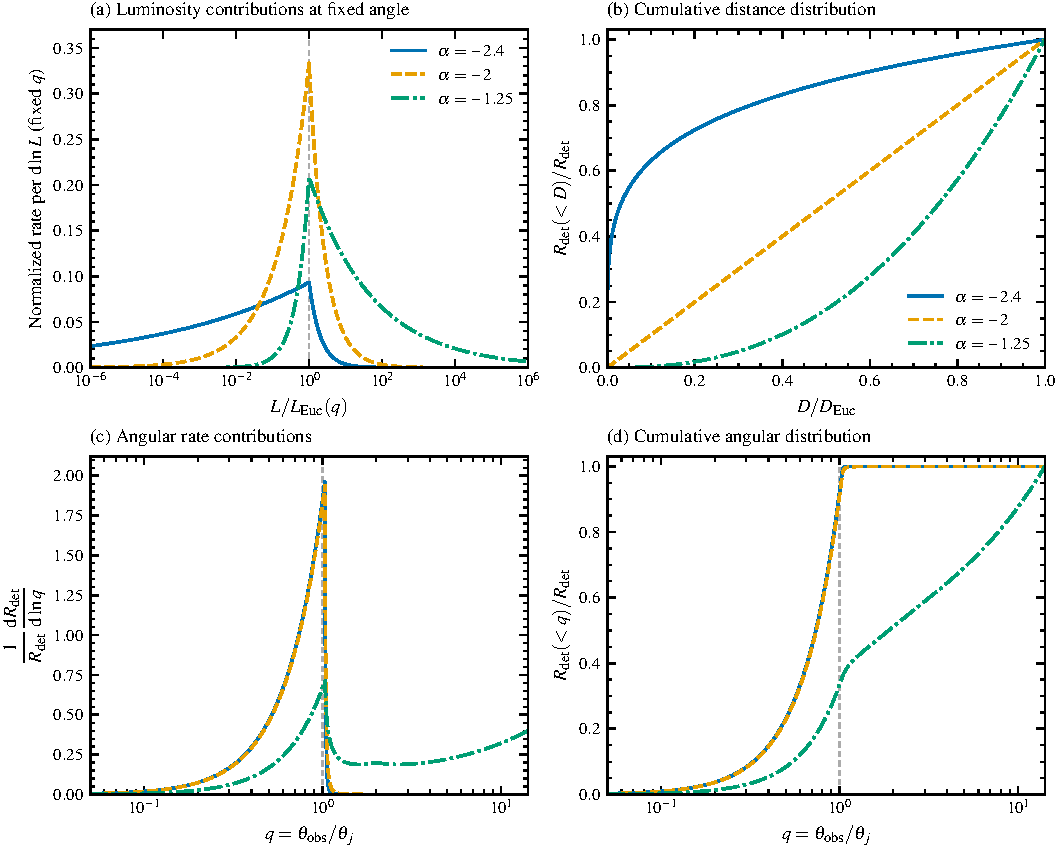
\includegraphics[width=\textwidth]{pedagogical_distributions.pdf}
\caption{General detected-population behavior for three LF slopes.
The luminosity panel is conditional on a fixed angle and uses its physical
threshold $L_\Euc(q)$. Its plotted range does not include all of the long
tails; normalization includes the full range $0<L<\infty$.
The distance distribution is independent of the light-curve shape.
The angular panels use continuous detection with $p=2.5$,
$\theta_j=0.1$, and $\Gamma_0=10^{2.5}$. Areas under logarithmic densities are taken
with respect to their logarithmic horizontal coordinates.}
\label{fig:distributions}
\end{figure}
\clearpage

\section{Explicit angular integration and the corner approximation}
\label{sec:angular}
Using the three branches of Eq.~\eqref{eq:threshold-branches}, the remaining
integral is
\begin{align}
 \int_0^{q_\nr}q\left(\frac{L_\Euc(q)}{\Lref}\right)^{\alpha+1}dq
 ={}&\frac{q_\dec^2}{2}\left(\frac{\Ldec}{\Lref}\right)^{\alpha+1}\notag\\
 &+\left(\frac{\Lj}{\Lref}\right)^{\alpha+1}
 \int_{q_\dec}^{2}q(q-1)^{2(p-1)(\alpha+1)}dq\notag\\
 &+\left(\frac{\Lj}{\Lref}\right)^{\alpha+1}
 \int_{2}^{q_\nr}q(q-1)^{2p(\alpha+1)}dq.
 \label{eq:angle-split}
\end{align}
To integrate, write $q=(q-1)+1$. Each integrand is then the sum of two
powers of $q-1$. Carrying out all three pieces gives the full rate:
\begin{equation}
\begin{aligned}
 \Rdet={}&\frac{4\pi\theta_j^2D_\Euc^3\mathcal A}
 {(-\alpha-1)(2\alpha+5)}\Bigg\{
 \frac{q_\dec^2}{2}\left(\frac{\Ldec}{\Lref}\right)^{\alpha+1}\\
 &+\left(\frac{\Lj}{\Lref}\right)^{\alpha+1}\Bigg[
 \frac{1-(q_\dec-1)^{2+2(p-1)(\alpha+1)}}{2+2(p-1)(\alpha+1)}\\
 &\hspace{3.9cm}+
 \frac{1-(q_\dec-1)^{1+2(p-1)(\alpha+1)}}{1+2(p-1)(\alpha+1)}\\
 &\hspace{3.9cm}+
 \frac{(q_\nr-1)^{2+2p(\alpha+1)}-1}{2+2p(\alpha+1)}\\
 &\hspace{3.9cm}+
 \frac{(q_\nr-1)^{1+2p(\alpha+1)}-1}{1+2p(\alpha+1)}
 \Bigg]\Bigg\}.
\end{aligned}
\label{eq:closed-rate}
\end{equation}
This expression is exact within the project's light curve and angular
geometry. It includes all luminosities and distances, as well as the
continuous transition across the jet break at $q=2$.

A denominator can vanish without the integral diverging. For the phase-II
terms this occurs at $\alpha=-1-1/(p-1)$ or
$\alpha=-1-1/[2(p-1)]$; replace the corresponding quotient by
$-\ln(q_\dec-1)$. For the phase-III terms it occurs at
$\alpha=-1-1/p$ or $\alpha=-1-1/(2p)$; replace the corresponding quotient
by $\ln(q_\nr-1)$. These are ordinary logarithmic integrals of
$(q-1)^{-1}$, with finite positive limits. They are unrelated to the
population-divergence boundaries $\alpha=-5/2$ and $\alpha=-1$.

\subsection{What is lost by retaining only the $q\simeq1$ region?}
Keeping only the constant-peak-flux core means retaining just the first
term in braces in Eq.~\eqref{eq:closed-rate}:
\begin{equation}
 R_{\rm det}(q\le q_\dec)=
 \frac{4\pi\theta_j^2D_\Euc^3\mathcal A}
 {(-\alpha-1)(2\alpha+5)}
 \frac{q_\dec^2}{2}\left(\frac{\Ldec}{\Lref}\right)^{\alpha+1}.
 \label{eq:core}
\end{equation}
Dividing this by the full rate gives exactly the detected fraction in that
core. Its complement is exactly the fractional rate omitted by this
approximation. This provides a direct accuracy measure rather than an
assumption of dominance. The geometrical on-axis region ends at $q=1$;
the constant-peak-flux core ends at the slightly larger $q_\dec$.

The thesis's most-contributing rectangle is a different approximation:
it changes its angle with luminosity. For $L<\Ldec$ it retains the core
out to its flux horizon; for $L>\Ldec$ it retains angles whose entire
Euclidean column is visible. Thus it keeps the core contribution and,
at every outer angle, only the luminosities above $L_\Euc(q)$.
Using Eq.~\eqref{eq:above-threshold} gives
\begin{equation}
 \frac{R_{\rm det}^{\rm rectangle}}{\Rdet}
 =1-\frac{2(-\alpha-1)}3
 \left[1-\frac{R_{\rm det}(q\le q_\dec)}{\Rdet}\right].
 \label{eq:rectangle}
\end{equation}
This explicitly separates the omitted outer-angle population from the
fraction of that population whose flux horizon is inside $D_\Euc$.
A good rectangle estimate does not by itself imply that most detections
have $q\simeq1$.


\section{How repeated detections change the threshold}
\label{sec:cadence}
\subsection{The thesis cadence approximation}
Let $t_+$ be the time at which the declining light curve falls below the
survey limit. For $i\ge2$, the thesis step approximation requires both a detectable peak
and $t_+\ge i\tcad$, after approximating the visible duration by $t_+$.
At $D_\Euc$, the latter condition requires
\begin{equation}
 L\ge L_i\equiv\frac{\Ldec}{\ft(i\tcad)}.
 \label{eq:Li}
\end{equation}
Writing it out in physical times,
\begin{equation}
 L_i=\begin{cases}
 \Ldec,&i\tcad\le\tdec,\\
 \Ldec(i\tcad/\tdec)^{3(p-1)/4},&\tdec<i\tcad<\tj,\\
 \Lj(i\tcad/\tj)^p,&\tj\le i\tcad<\tnr,\\
 \Lnr(i\tcad/\tnr)^{(15p-21)/10},&i\tcad\ge\tnr.
 \end{cases}
 \label{eq:Li-explicit}
\end{equation}
Peak detection requires $L\ge L_\Euc(q)$; repeated detection in this
approximation requires $L\ge L_i$. The actual threshold is therefore
\begin{equation}
 \boxed{L\ge\max[L_\Euc(q),L_i]\quad\hbox{at }D_\Euc.}
 \label{eq:cad-threshold}
\end{equation}
At a smaller distance, multiply that threshold by $(D/D_\Euc)^2$.
The derivation of the previous sections consequently applies with the
explicit replacement
$L_\Euc(q)\longrightarrow\max[L_\Euc(q),L_i]$:
\begin{equation}
 R_{\ge i}^{\rm thesis}=
 \frac{4\pi\theta_j^2D_\Euc^3\mathcal A}
 {(-\alpha-1)(2\alpha+5)}
 \int_0^{q_\nr}q
 \left(\frac{\max[L_\Euc(q),L_i]}{\Lref}\right)^{\alpha+1}dq.
 \label{eq:cad-rate}
\end{equation}
The convergence interval and the exact $\Flim$ and $D_\Euc$ scalings are
unchanged. The luminosity and angle distributions change because the
physical threshold has changed.

The angle $q_i$ at which the two constraints agree satisfies
$t_p(q_i)=i\tcad$, hence
\begin{equation}
 q_i=\begin{cases}
 1+(i\tcad/\tj)^{3/8},&\tdec<i\tcad<\tj,\\
 1+(i\tcad/\tj)^{1/2},&\tj\le i\tcad<\tnr.
 \end{cases}
 \label{eq:qi}
\end{equation}
For $q<q_i$ the common threshold is $L_i$; for $q>q_i$ it is
$L_\Euc(q)$. The candidate most-contributing point therefore moves from
$(q_\dec,D_\Euc)$ at luminosity $\Ldec$ to
$(q_i,D_\Euc)$ at luminosity $L_i$. In particular, $q_i$ need not be close
to one.

\subsection{The cadence integral is still analytic}
For $q_\dec<q_i<2$, Eq.~\eqref{eq:closed-rate} applies after replacing
$q_\dec$ by $q_i$ in the angular limits and replacing $\Ldec$ by $L_i$
in the core term; $\Lj$ is unchanged. This directly performs all the
integrals in Eq.~\eqref{eq:cad-rate}.
For $2\le q_i<q_\nr$, the phase-II integral is absent and the result is
\begin{equation}
\begin{aligned}
 R_{\ge i}^{\rm thesis}={}&
 \frac{4\pi\theta_j^2D_\Euc^3\mathcal A}
 {(-\alpha-1)(2\alpha+5)}\Bigg\{
 \frac{q_i^2}{2}\left(\frac{L_i}{\Lref}\right)^{\alpha+1}\\
 &+\left(\frac{\Lj}{\Lref}\right)^{\alpha+1}\Bigg[
 \frac{(q_\nr-1)^{2+2p(\alpha+1)}-(q_i-1)^{2+2p(\alpha+1)}}
 {2+2p(\alpha+1)}\\
 &\hspace{3.5cm}+
 \frac{(q_\nr-1)^{1+2p(\alpha+1)}-(q_i-1)^{1+2p(\alpha+1)}}
 {1+2p(\alpha+1)}\Bigg]\Bigg\}.
\end{aligned}
\label{eq:cad-closed}
\end{equation}
A zero denominator again gives the logarithm
$\ln[(q_\nr-1)/(q_i-1)]$ for the relevant quotient.
For $i\tcad\le\tdec$ the continuous result is recovered.
For $i\tcad\ge\tnr$, all angles are time limited and the integral in
Eq.~\eqref{eq:cad-rate} is simply
$(q_\nr^2/2)(L_i/\Lref)^{\alpha+1}$.

There is no single cadence power law valid across all these cases.
In phase III, if $1\ll q_i\ll q_\nr$ and
$-p(\alpha+1)>1$, the outer-angle integral is dominated by its lower
limit and the rate scales approximately as
\begin{equation}
 R_{\ge i}^{\rm thesis}\propto(i\tcad)^{1+p(\alpha+1)}.
 \label{eq:cad-asymptote}
\end{equation}
The extra power of one comes from $q_i^2\propto i\tcad$;
the other factor comes from $L_i^{\alpha+1}\propto(i\tcad)^{p(\alpha+1)}$.
The conditions matter: near the jet break, near the outer angular boundary,
or for a shallow luminosity function, the explicit expression must be used.
At fixed shape, increasing the required duration cannot increase the exact
rate, because it only raises the threshold in Eq.~\eqref{eq:cad-rate}.

\subsection{Retaining the peak time and the random observing phase}
The physical visible duration is $\Delta t_{\rm det}=t_+-t_p(q)$ when
positive. In a periodic sequence of instantaneous visits, the next visit
occurs at a uniformly random time between $t_p(q)$ and $t_p(q)+\tcad$.
The time of the $i$th visit is therefore uniform between
$t_p(q)+(i-1)\tcad$ and $t_p(q)+i\tcad$.
The project probability ramp follows:
\begin{equation}
 P_{\ge i}=\begin{cases}
 0,&\Delta t_{\rm det}<(i-1)\tcad,\\
 \Delta t_{\rm det}/\tcad-(i-1),
       &(i-1)\tcad\le\Delta t_{\rm det}<i\tcad,\\
 1,&\Delta t_{\rm det}\ge i\tcad.
 \end{cases}
 \label{eq:ramp}
\end{equation}
At a specified time $t$ of that $i$th visit, the required luminosity at
$D_\Euc$ is $\Ldec/\ft(t)$. Integrating the luminosity and distance exactly
as before, then averaging over the visit time, gives
\begin{equation}
\begin{aligned}
 R_{\ge i}^{\rm random\ phase}={}&
 \frac{4\pi\theta_j^2D_\Euc^3\mathcal A}
 {(-\alpha-1)(2\alpha+5)}
 \int_0^{q_\nr}q\,dq\,\frac1{\tcad}\\
 &\quad\times\int_{t_p(q)+(i-1)\tcad}^{t_p(q)+i\tcad}
 \left(\frac{\Ldec}{\Lref\ft(t)}\right)^{\alpha+1}dt.
\end{aligned}
\label{eq:random-phase}
\end{equation}
The time integral is a power or logarithm on each temporal branch; its
explicit primitives are given in Appendix~\ref{app:time}.
Splitting at $\tj$ and $\tnr$ handles visits crossing a transition.
The final angular integral can then be evaluated by one-dimensional
quadrature. No additional luminosity or distance quadrature is needed.

Since the light curve decreases, evaluating the inner integrand at its
latest endpoint gives a lower bound on its average; evaluating it at its
earliest endpoint gives an upper bound. These are the two peak-retained
step bounds on the random-phase rate. The thesis step instead uses the
threshold time $\max[t_p(q),i\tcad]$. It is a different approximation,
so there is no general ordering between it and the random-phase result.
For $i=1$, peak detectability alone is not enough for a periodic visit to
catch the event. As $\tcad\to0$ at fixed $i$, Eq.~\eqref{eq:random-phase}
recovers continuous detection.

Crucially, the visit times depend on angle and cadence but not on $D$ or $L$.
The distance factor in Eq.~\eqref{eq:L-first} is therefore unchanged:
all these prescriptions share Eq.~\eqref{eq:distance-cdf}.
The same is true for any selection depending on flux, viewing angle, and
timing, provided it introduces no separate luminosity or distance scale
and has nonzero finite selected weight. Two such surveys can have different
rates and luminosity distributions while predicting the same normalized
distance distribution.

\begin{figure}[H]
\centering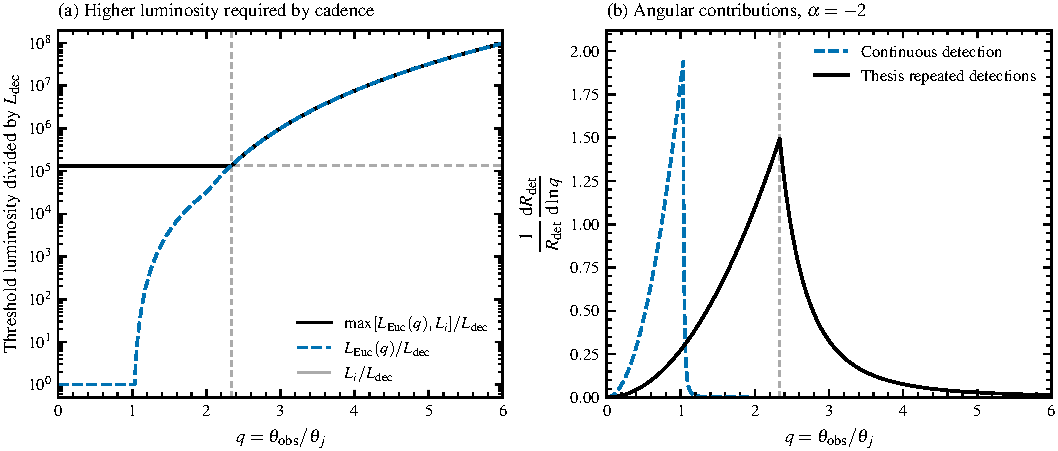
\includegraphics[width=\textwidth]{pedagogical_cadence.pdf}
\caption{How repeated detections alter the threshold and viewing angles.
The thesis step replaces $L_\Euc(q)$ by $\max[L_\Euc(q),L_i]$.
Using the shape in Figure~\ref{fig:distributions}, $\tdec=19.4$ s,
$\alpha=-2$, $i=2$, and a two-day cadence, the angular contribution rises
to the shifted corner at $q_i=2.335$. These curves illustrate the analytic
step construction, not a precision selection model for a particular survey.}
\label{fig:cadence}
\end{figure}

\section{Relation to the original bounded luminosity function}
\label{sec:bounded}
\subsection{Match the differential normalization, not the total rate}
For the same intensity restricted to $L_{\min}\le L\le L_{\max}$,
the finite intrinsic rate density is
\begin{equation}
 \mathcal R_{[L_{\min},L_{\max}]}=
 \frac{\mathcal A}{\alpha+1}
 \left[\left(\frac{L_{\max}}{\Lref}\right)^{\alpha+1}
      -\left(\frac{L_{\min}}{\Lref}\right)^{\alpha+1}\right].
 \label{eq:bounded-normalization}
\end{equation}
The normalized distribution used by the previous model is
\begin{equation}
 \phi(L)=\frac{(\alpha+1)L^\alpha}
 {L_{\max}^{\alpha+1}-L_{\min}^{\alpha+1}},
 \qquad L_{\min}\le L\le L_{\max}.
 \label{eq:bounded-pdf}
\end{equation}
Equations~\eqref{eq:bounded-normalization} and \eqref{eq:bounded-pdf}
satisfy $\mathcal R_{[L_{\min},L_{\max}]}\phi(L)=d\mathcal R/dL$.
The previous total rate inside the Euclidean sphere is then
$R_{\rm int}=(4\pi/3)D_\Euc^3\mathcal R_{[L_{\min},L_{\max}]}$.
At $\alpha=-1$, the intrinsic normalization is instead
$\mathcal A\ln(L_{\max}/L_{\min})$ and
$\phi(L)=1/[L\ln(L_{\max}/L_{\min})]$.

The correct infinite-range limit holds $\mathcal A$ fixed while moving the
bounds outward. The finite total intrinsic rate must then change.
Holding $R_{\rm int}$ fixed while lowering $L_{\min}$ would reduce the
number of events at every fixed detectable luminosity for $\alpha<-1$.
That procedure tests a changing population, not convergence to the
simplified intensity.

\subsection{How rapidly do finite-cutoff results approach this model?}
Suppose first that $L_{\min}<L_\Euc(q)<L_{\max}$ at a given angle.
Integrating the two sides of Eq.~\eqref{eq:split-L} with finite limits gives
\begin{equation}
\begin{aligned}
 \frac{dR_{\rm det}^{\rm bounded}}{dq}={}&
 \frac{4\pi\theta_j^2D_\Euc^3\mathcal A}{3}\,q
 \left(\frac{L_\Euc(q)}{\Lref}\right)^{\alpha+1}\\
 &\times\left[
 \frac{1-(L_{\min}/L_\Euc(q))^{\alpha+5/2}}{\alpha+5/2}
 +\frac{1-(L_{\max}/L_\Euc(q))^{\alpha+1}}{-\alpha-1}\right].
\end{aligned}
\label{eq:bounded-rate}
\end{equation}
If both bounds lie below $L_\Euc(q)$, only the unsaturated volume branch
is present. If both lie above it, only the fully visible branch is present.
In either case the original volume integral, Eq.~\eqref{eq:volume}, gives
the appropriate finite limits without extrapolating Eq.~\eqref{eq:bounded-rate}.

For a threshold between the bounds, the fractional contributions excluded
by the lower and upper cutoffs are respectively
\begin{align}
 \frac{dR_{\rm det}(L<L_{\min})/dq}{d\Rdet/dq}
 &=\frac{2(-\alpha-1)}3
 \left(\frac{L_{\min}}{L_\Euc(q)}\right)^{\alpha+5/2},
 \label{eq:faint-tail}\\
 \frac{dR_{\rm det}(L>L_{\max})/dq}{d\Rdet/dq}
 &=\frac{2(\alpha+5/2)}3
 \left(\frac{L_{\max}}{L_\Euc(q)}\right)^{\alpha+1}.
 \label{eq:bright-tail}
\end{align}
These follow equally from the conditional CDF. Their detected angular-weighted
average is the fractional error in the total rate. For cadence, use
$\max[L_\Euc(q),L_i]$; for random phase, also average over the selected
visit times.

The tail powers approach zero at the convergence boundaries, so even very
remote cutoffs can then matter. At $\alpha=-5/2$, the faint integral is
proportional to $\ln[L_\Euc(q)/L_{\min}]$; at $\alpha=-1$, the bright
integral is proportional to $\ln[L_{\max}/L_\Euc(q)]$.
Outside the convergent interval the divergence is a power of the corresponding
cutoff. There is no cutoff-independent detected-rate limit there.

\subsection{What changes in the dependence on survey depth?}
A bounded population has two limiting behaviors at fixed cadence and shape.
If the survey is so shallow that all its luminosities have horizons inside
$D_\Euc$, the volume factor gives $R_{\rm det}^{\rm bounded}\propto\Flim^{-3/2}$.
If it is so deep that every luminosity at every included angle fills the
Euclidean volume, the rate is independent of $\Flim$.
In between, some luminosity--angle pairs are unsaturated and others are
already visible throughout the volume.

Differentiating Eq.~\eqref{eq:volume} makes this precise. Only its unsaturated
branch depends on $\Flim$, with logarithmic derivative $-3/2$.
The moving-boundary terms cancel because both volume branches agree at
$L=L_\Euc(q)$. Thus, for a fixed bounded population under continuous detection,
\begin{equation}
 \frac{d\ln R_{\rm det}^{\rm bounded}}{d\ln\Flim}
 =-\frac32\,
 \frac{R_{\rm det}^{\rm bounded}(L<L_\Euc(q))}
 {R_{\rm det}^{\rm bounded}}.
 \label{eq:bounded-flux-slope}
\end{equation}
The numerator counts the part of the selected rate whose flux horizon is
inside the volume, integrating over both luminosity and angle. In the
unbounded power law its fraction is the same at every angle,
$2(-\alpha-1)/3$, from Eq.~\eqref{eq:below-threshold}. Consequently
Eq.~\eqref{eq:bounded-flux-slope} reduces exactly to the slope $\alpha+1$.
For the thesis cadence step the same derivation uses the unsaturated condition
$L<\max[L_\Euc(q),L_i]$.

This explains the simplification physically. A bounded LF moves through
shallow, intermediate, and saturated survey regimes. An unbounded power law
always supplies fainter and brighter events around the current threshold,
so the balance between unsaturated and saturated contributions stays fixed.
Its single exact flux power law describes the intermediate behavior when
both real luminosity bounds are sufficiently remote; it cannot reproduce
the two eventual cutoff-controlled limits.

\section{A few illustrations and the limits of the approximation}
\label{sec:examples}
Table~\ref{tab:illustrations} uses only the analytic expressions above.
It does not require an afterglow parameter set or a calibrated normalization.
The contrast between a mode and an enclosed fraction is already visible.
\begin{table}[H]
\centering
\caption{Dimensionless examples from Eqs.~\eqref{eq:below-threshold},
\eqref{eq:Lmedian}, and \eqref{eq:distance-cdf}. Luminosity statements are
conditional on a fixed viewing angle; the distance median is global.}
\label{tab:illustrations}
\begin{tabular}{@{}rrrr@{}}
\toprule
$\alpha$ & $L_{\mathrm{med}\mid q}/L_\Euc(q)$
 & $\Pr(L<L_\Euc(q)\mid q,\mathrm{detected})$ & $D_{\rm med}/D_\Euc$\\
\midrule
$-2.4$ & $0.00195$ & $0.933$ & $0.03125$\\
$-2$   & $0.5625$  & $0.667$ & $0.500$\\
$-1.25$ & $7.716$ & $0.167$ & $0.758$\\
\bottomrule
\end{tabular}
\end{table}
For the steeper slope the threshold remains the conditional logarithmic
maximum, yet most detections are much fainter and closer than that threshold
might suggest. For the shallower slope most events at each angle are above
the local threshold. Their typical luminosity grows further when more
off-axis angles, with larger thresholds, contribute.

Figure~\ref{fig:distributions} adds the project's illustrative shape
$p=2.5$, $\theta_j=0.1$, $\Gamma_0=10^{2.5}$, and $\tdec=19.4$ s.
At $\alpha=-2$, about $96.9\%$ of continuously detected events lie within
$q_\dec=1.0316$. Thus this case supports the angular-core approximation,
while its distance median is still only $D_\Euc/2$.
With two required detections separated by two days, the same shape gives
$q_i=2.335$ and $L_i/\Ldec\simeq1.34\times10^5$.
Figure~\ref{fig:cadence} illustrates why the original $q\simeq1$ threshold
is then no longer the relevant repeated-detection threshold.


Retaining the peak and averaging phase need not be a small correction to
the thesis step. For this same two-day example at $\alpha=-2$, the rate is
about $14\%$ higher for two required visits, but about $48\%$ lower for ten
required visits. The change of sign illustrates why a universal correction
factor is unsuitable. These are examples of the distinction between timing
prescriptions, not fitted observational results.

The analytic calculations were checked against independent quadrature,
including the logarithmic cases, CDF normalization, recovered medians, and
reference-luminosity invariance. Smooth controlled checks agree to better
than the target relative accuracy $10^{-7}$. Finite-cutoff calculations
matched to the unchanged bounded-LF engine agree within $0.042\%$ in rate
and $0.025\%$ in distance median for the stored reference cases, comfortably
inside the one-percent criterion. Those comparisons keep the differential
normalization fixed as the bounds move.
The numerical tests, resolution studies, and the earlier ZTF benchmark
remain in the accompanying analysis files; their detailed tables are not
needed for this derivation.

\section{What can be taken into the paper?}
The two-parameter intensity gives a closed detected-rate calculation because
the detectable volume rises as $L^{3/2}$ and then saturates. Those two
behaviors yield the convergence interval, the exact flux law, and the two
sides of the detected luminosity distribution directly.

The threshold $\Ldec=4\pi D_\Euc^2\Flim$ has a precise role: it is the
conditional logarithmic maximum within the full-time angular core.
Calling it the characteristic detected luminosity additionally requires
checking the breadth of the distribution and the contribution of other
angles. Cadence changes that threshold to $L_i$ within $q_i$, and the
random-phase construction gives a controlled way to retain the peak time.

The distance prediction is especially restrictive. At fixed $\alpha$ and
$D_\Euc$, changes in survey depth and homogeneous timing selection do not
change the normalized distance distribution. The bounded model can depart
from this prediction when a luminosity cutoff becomes relevant. This
provides a general comparison between the models, separate from any
particular normalization or survey benchmark.

The simplification is therefore useful as a controlled description of the
detected population when omitted luminosity tails are small. It is not a
complete intrinsic population model. The explicit tail fractions identify
when physical cutoffs can be ignored and when they must be restored.

\appendix
\section{Explicit time integrals for random-phase detection}
\label{app:time}
To evaluate Eq.~\eqref{eq:random-phase}, split its physical time interval
at $\tj$ and $\tnr$. If the two endpoints $t_1,t_2$ lie within phase II,
\begin{equation}
 \int_{t_1}^{t_2}\left(\frac{\Ldec}{\Lref\ft(t)}\right)^{\alpha+1}dt
 =\tdec\left(\frac{\Ldec}{\Lref}\right)^{\alpha+1}
 \frac{(t_2/\tdec)^{1+3(p-1)(\alpha+1)/4}
 -(t_1/\tdec)^{1+3(p-1)(\alpha+1)/4}}
 {1+3(p-1)(\alpha+1)/4}.
 \label{eq:time-II}
\end{equation}
Within phase III the same integral is
\begin{equation}
 \int_{t_1}^{t_2}\left(\frac{\Ldec}{\Lref\ft(t)}\right)^{\alpha+1}dt
 =\tj\left(\frac{\Lj}{\Lref}\right)^{\alpha+1}
 \frac{(t_2/\tj)^{1+p(\alpha+1)}-(t_1/\tj)^{1+p(\alpha+1)}}
 {1+p(\alpha+1)}.
 \label{eq:time-III}
\end{equation}
Within phase IV it is
\begin{equation}
 \int_{t_1}^{t_2}\left(\frac{\Ldec}{\Lref\ft(t)}\right)^{\alpha+1}dt
 =\tnr\left(\frac{\Lnr}{\Lref}\right)^{\alpha+1}
 \frac{(t_2/\tnr)^{1+(15p-21)(\alpha+1)/10}
 -(t_1/\tnr)^{1+(15p-21)(\alpha+1)/10}}
 {1+(15p-21)(\alpha+1)/10}.
 \label{eq:time-IV}
\end{equation}
When the denominator of one expression vanishes, replace that expression
by, respectively,
\begin{equation}
 \tdec(\Ldec/\Lref)^{\alpha+1}\ln(t_2/t_1),\qquad
 \tj(\Lj/\Lref)^{\alpha+1}\ln(t_2/t_1),\qquad
 \tnr(\Lnr/\Lref)^{\alpha+1}\ln(t_2/t_1).
 \label{eq:time-log}
\end{equation}
These are finite-interval logarithmic limits. The Newtonian branch changes
the timing weight when a required visit crosses $\tnr$; it does not change
the luminosity--distance convergence interval.

\section{Source conventions and reproducibility}
The thesis and the previous LF derivation set the notation. The following
source discrepancies are resolved using the physical light curve:
\begin{enumerate}
\item The jet-break threshold follows from the decreasing peak flux:
$\widetilde F_{\rm lim,j}=(\Gamma_0\theta_j)^{-2(p-1)}$.
This corrects the sign in thesis Eq.~45.
\item The phase-III light curve can also be written as
$\ft(t)=(\tj/\tdec)^{(p+3)/4}(t/\tdec)^{-p}$.
This fixes the jet-time factor in thesis Eq.~69.
\item The single-luminosity phase-III cadence factor contains
$(i\tcad/\tj)^{-3p/2}[1+(i\tcad/\tj)^{1/2}]^2$.
Its large-duration power is $1-3p/2$, not $-3(p-2)/2$.
Equation~\eqref{eq:cad-asymptote} is the separate LF-integrated asymptote.
\item The probability of one visit is
$\min(\Delta t_{\rm det}/\tcad,1)$, following the thesis ramp.
A printed maximum that exceeds unity cannot be used as a probability.
\item The reference engine continues phase III in its timing inversion;
the thesis includes the Newtonian branch. Equation~\eqref{eq:lightcurve}
uses the thesis branch. Finite-cutoff engine checks compare matching timing
conventions, and the separate late-time calculations retain this distinction.
\end{enumerate}

For comparisons to the application's one-day luminosity, use
\begin{equation}
 \nu L_\nu(1\,\mathrm{day})=\nu\ft(1\,\mathrm{day})L_\nu(\tdec).
 \label{eq:oneday}
\end{equation}
The broken light curve is essential if the jet break precedes one day.
This linear transformation preserves $\alpha$, but the luminosity limits
and normalization must refer to consistent units and epochs.

Calculations, tests, and rebuild instructions are in
\path{analysis/simplified_luminosity_function/}. The app and engine are unchanged.

\begingroup\small
\begin{thebibliography}{9}
\bibitem{Thesis} Bachelor's project, \emph{Detection Rates of Gamma-Ray Burst
Afterglows in Optical Surveys -- An Analytic Approach}. Local source in
\texttt{sources/}; especially Eqs.~21, 32--40, 45--53, 60, 63--77 and Figure~15.
\bibitem{PreviousLF} \emph{Detection Rates of GRB Afterglows with a Luminosity
Distribution}. Project derivation, September 2026,
\texttt{docs/luminosity\_function\_derivation.tex}.
\end{thebibliography}
\endgroup
\end{document}

